\chapter{Wstęp i motywacja}

%\section*{Opis rozdziału}
%
%W tym rozdziale streszczono główną koncepcję związaną z \MZM.
%Zamieszczono również informację dotyczącą pierwszych eksperymentów, które 
%starają udowodnić istnienie quasicząstek Majorany, a także aktualny postęp prac teoretycznych.

\section{Wprowadzenie}

Pojęcie {\it cząstek Majorany} po raz pierwszy pojawiło się  w latach 30 \Romanbar{XX} wieku, gdy Ettore Majorana otrzymał rzeczywiste rozwiązanie równania Diraca~\cite{dirac.1928}.
Konsekwencją tego była nierozróżnialność cząstki i jej antycząstki~\cite{majorana.1937}.
Niestety w fizyce wysokich energii nie udało się potwierdzić istnienia fermionów Majorany.
%Potencjalnymi kandydatami dla takich rzeczywistych cząstek, w fizyce wysokich energii, są m.in. neutrina~\cite{avignone.elliott.2008,rodejohann.2011} czy zimna ciemna materia~\cite{pawlak.hoffman.2019} {\bf to zdanie jest IMO zbedne - ale jesli sie upierasz to chociaz daj ref do orYginalnych prac a nie prac przegladowych}.
Okazuje się jednak, że w fizyce ciała stałego istnieją stany, tzw. quasiczątek, które posiadają analogiczne cechy do fermionów Majorany. 

\subsection*{Model Kitaeva}

Koncepcja fermionów Majorany odrodziła się we współczesnej fizyce ciała stałego dzięki przełomowej pracy A.~Y.~Kitaeva~\cite{kitaev.2001}. 
W tej pracy, bazując na modelu bezpinowych fermionów w~jednowymiarowym (1D) otwartym łańcuchu z parowaniem międzywęzłowym\footnote{Szczegółowy opis modelu Kitaeva został przedstawiony w~rozdziale~\ref{chap:majorana}.}, Kitaev przedstawił koncepcję realizacji stanów brzegowych.
Te stany, ze względu na swoje cechy takie jak nierozróżnialność, przez analogię do fermionów Majorany nazywane są aktualnie \textit{stanami Majorany} lub \textit{stanami Majorany o zerowej energii} (z ang. \textit{Majorana Zero Mode},~\MZM).
Praca ta zainspirowała liczne badania teoretyczne, jak i eksperymentalne~\cite{nayak.simon.2008,beenakker.2013,elliott.franz.2015,lutchyn.bakkers.2018,pawlak.hoffman.2019}.
Postęp technik eksperymentalnych umożliwił poszukiwania \MZM\ w różnych układach, takich jak np. monoatomowe łańcuchy magnetyczne na powierzchni nadprzewodnika czy nanostruktury hybrydowe półprzewodnik--nadprzewodnik.
Należy tutaj wspomnieć, że koncepcja \MZM\ stanowi ciągle aktualną tematykę badawczą. 
W dniu 8 grudnia 2019 roku, na serwisie \texttt{\normalsize arXiv} można było  znaleźć blisko 3000 preprintów w kategorii \texttt{\normalsize cond-mat} ze słowem kluczowym ,,Majorana'',
natomiast wyszukiwarka \texttt{\normalsize Google Scholar} znalazła 32100 wystąpienia hasła ,,Majorana zero modes''.
To żywe zainteresowanie wynika z chęci wykorzystania \MZM\ w~praktycznych zastosowaniach, takich jak obliczenia kwantowe.

\subsection*{Własności MZM}

Zainteresowanie \MZM\ jest głównie związane z ich egzotycznymi własnościami, wśród których warto  wymienić:
\begin{enumerate}

\item \textit{Lokalizacja na krawędzi.}
\MZM, jako stany brzegowe, mogą być uzyskane jedynie w~układzie, który posiada ,,krawędź''.
Jest to sytuacja analogiczna do modelu Kitaeva, gdzie przy pewnych parametrach modelu, \MZM\ są zlokalizowane dokładnie na ostatnich węzłach otwartego łańcucha.
Badania teoretyczne sugerują, że w rzeczywistych układach niskowymiarowych, \MZM\ są zlokalizowane na długości od kilku do kilkunastu stałych sieciowych.

\item \textit{Nierozróżnialność ,,cząstki'' i ,,antycząstki''.}
W realistycznych układach \MZM\ mogą być realizowane poprzez synergię nadprzewodnictwa, sprzężenia spin--orbita oraz zewnętrznego pola magnetycznego.
Wpływ nadprzewodnictwa, z uwagi na obecną symetrię cząstka--dziura, implikuje istnienie par quasicząstek o przeciwnych energiach~\cite{wilczek.2009,chamon.jackiw.2010,leijnse.flensberg.2012,beenakker.2014,sato.yoichi.2017}.
W konsekwencji, quasicząstka i jej antycząstka są nierozróżnialne gdy posiadają tę samą energię, tj. energię równą zero (znajdują się na poziomie Fermiego).

\item \textit{Ochrona topologiczna.}
\MZM\ są realizowane jako stany brzegowe o zerowej energii.
Oznacza to, że pomiędzy energią \MZM, a energią kolejnych wzbudzeń quasicząstek, musi istnieć przerwa energetyczna o niezerowej wartości (tzw. {\it przerwa topologiczna}).
Taka szczelina gwarantuje, że \MZM\ są niewrażliwe na zewnętrzne czynniki, tj. nieporządek --- tę cechę nazywamy ochroną topologiczną.

\item \textit{Anyony.}
Okazuje się, że \MZM\ nie podlegają statystyce Fermiego--Diraca, ani Bosego--Einsteina, tzn. nie są ani fermionami, ani bozonami --- takie obiekty nazywamy {\it anyonami} ({\it any-} z ang. ,,jakikolwiek'')~\cite{read.green.2000,ivanov.2001,nayak.simon.2008,lahtinen.pachos.2017}.
W odróżnieniu od fermionów czy bozonów, zamiana miejscami dwóch anyonów prowadzi do nietrywialnej transformacji stanu kwantowego układu.%
\footnote{Szczegółowe omówienie tego zjawiska wraz z~zastosowaniem do tzw. operacji wyplatania (ang. \textit{braiding})  można znaleźć w~rozdziale~\ref{chap:topologicalQuantumComputing}.}
%Oznacza to, że przy zamianie miejscami dwóch \MZM, stan układu zmienia swoją fazę o dowolny czynnik ({\it any} z ang. ,,jakikolwiek''), a nie o czynnik $\pm1$ jak w przypadku fermionów czy bozonów.
%{\color{red} AW: ja bym tutaj nie pisał o fazach! na  tel powiem}

\item \glslink{NAS}{Statystyka nieabelowa (NAS, ang. non-Abelian statistics).}
Anyony możemy podzielić na dwie kategorie~\cite{bhattacharjee.mj.2017}: abelowe oraz nieabelowe, w zależności czy kolejność wymiany cząstek ma znaczenie na stan układu lub nie~\cite{lahtinen.pachos.2017}.
Wymiana zorientowana zgodnie ze wskazówkami zegara będzie miała inny wpływ na stanu układu, niż wymiana zorientowana przeciwnie.
Należy tutaj podkreślić, że nieabelowość \MZM\ to cecha występująca tylko i wyłącznie w niskowymiarowych układach.
Tej cechy nie posiadają natomiast fermiony Majorany w fizyce cząstek elementarnych w przestrzeni trójwymiarowej.

\end{enumerate}

Ze względu na wymienione cechy, \MZM\ są bardzo atrakcyjnymi obiektami do potencjalnego zastosowania w komputerach kwantowych. 
Dzięki ochronie topologicznej oraz statystyce nieabelowej, \MZM\ mogą pełnić rolę podstawowego budulca w topologicznych komputerach kwantowych~\cite{kitaev.2003,sarma.freedman.2005,nayak.simon.2008,stanescu.2016,field.simula.2018} (dokładniej zostanie to omówione w rozdziale~\ref{chap:topologicalQuantumComputing}).
Do realizacji takiego komputera potrzebne są bity kwantowe (qubity) oraz możliwe operacje na tych qubitach.
Rolę qubitów mają pełnić tu \MZM, a operacji na qubitach poszczególne operacje wymiany pomiędzy \MZM.
Dzięki \textit{ochronie topologicznej}, operacje jak i dane byłyby niewrażliwe na zaburzenia zewnętrzne~\cite{nayak.simon.2008, hasan.kane.2010, beenakker.2013, elliott.franz.2015, beenakker.2019}, 
%tak długo jak energia wzbudzeń znajduje się powyżej szczeliny energetycznej wynikającej z nadprzewodnictwa oraz tak długo jak zachowana jest symetria parzystości układu, która jest wymagana do istnienia \MZM\ ~\cite{cheng.lutchyn.2012}.
tak długo jak przerwa energetyczna pomiędzy energią stanów podstawowych, a energią stanów wzbudzonych jest dostatecznie duża oraz zachowana jest symetria parzystości niezbędna do istnienia \MZM\ ~\cite{cheng.lutchyn.2012}.

Konstrukcja komputera kwantowego z wykorzystaniem \MZM\ nie gwarantuje jednak uniwersalności obliczeń, ale sam fakt wykonywania części operacji z zagwarantowaną ochroną topologiczną motywuje fizyków do dalszych badań.
%O potencjalnym wykorzystaniu komputerów kwantowych można by napisać oddzielną rozprawę.
Ostatnie raporty dotyczące wysycania \textit{prawa Moore'a}~\cite{moore.1965} szczególnie zasługują tutaj na uwagę, gdyż oznaczają zbliżanie się do granicy miniaturyzacji komputerów klasycznych.
%Postęp technologiczny miniaturyzacji układów scalonych osiąga swoje maksymalne możliwości, ale nadzieja leży w~komputerach kwantowych, które mogą stać się nowym napędem technologicznym ludzkości.
Dalszy postęp w technikach komputerowych, może być więc realizowany poprzez komputery nowej klasy.
Zagadnienie to jednak wykracza poza zakres prezentowanej rozprawy doktorskiej.

\subsection*{Realistyczne modele}

Założenia modelu Kitaeva uniemożliwiają jego realizację w układach ciała stałego.
Wynika to z faktu realizacji w tym modelu parowania typu~\emph{p} w układach bezspinowych fermionów.
Okazuje się jednak, że w pewnym zakresie parametrów, takich jak pole magnetyczne czy potencjał chemiczny, układy 1D sprzężone z nadprzewodnikiem mogą realizować podobny scenariusz.
W takim przypadku, faza topologiczna uzyskiwana jest przez wzajemny wpływ sprzężenia spin--orbita (\acrshort{SO}), nadprzewodnictwa oraz zewnętrznego pola magnetycznego~\cite{alicea.2012,kiczek.ptok.2017,lutchyn.bakkers.2018}.
%Omówmy pokrótce wpływ każdego z tych czynników.
Sprzężenie \acrshort{SO} znosi degenerację spinową początkowo parabolicznej relacji dyspersyjnej, natomiast pole magnetyczne powoduje otwarcie szczeliny w punkcie $k = 0$ --- rysunek~\ref{fig:intro1}(a) (zaczerpnięty z pracy~\cite{lutchyn.bakkers.2018}).
Jeśli poziom Fermiego (reprezentowany tutaj przez $\muuniform$) przecina jedynie jedną z gałęzi pasm (jak pokazano na schemacie), to wyindukowane nadprzewodnictwo występuje pomiędzy quasicząstkami w ramach jednego pasma -- układ znajduje się w fazie topologicznej oraz efektywnie realizowane jest parowanie typu $p$.
W przeciwnym przypadku, parowanie następuje pomiędzy dwoma gałęziami i układ znajduje się w fazie trywialnej topologicznie.


Okazuje się, że zakres parametrów, gdzie faza topologiczna może być realizowana, jest ściśle określony przez parametry układu takie jak: wyindukowana szczelina nadprzewodząca $\DeltaSCuniform_0$ oraz potencjał chemiczny $\muuniform$ (inaczej: położenie poziomu Fermiego). 
\MZM\ w skończonym układzie, mogą być realizowane gdy układ znajduje się w fazie nietrywialnej topologicznie, przy czym przejście z fazy trywialnej do nietrywialnej jest określone przez pole magnetyczne $\zeeman$ --- rysunek~\ref{fig:intro1}(b) (zaczerpnięty z pracy~\cite{lutchyn.bakkers.2018}).
Granica fazy topologicznej jest tutaj dana poprzez pewne pole krytyczne $V_Z^c = \sqrt{ \muuniform^2 + \DeltaSCuniform_0^2 }$~\cite{sato.2006,sato.fujimoto.2009,sato.takahashi.2009,sato.takahashi.2010} i przyjmuje postać ,,paraboli'' na diagramie fazowym.
W polu magnetycznym $V_Z^c$ następuje zamknięcie trywialnej szczeliny nadprzewodzącej (np. wyindukowanej poprzez efekt bliskości) i otwarcie nowej szczeliny topologicznej, chroniącej \MZM~\cite{lutchyn.bakkers.2018}.


\begin{figure}
    \centering
    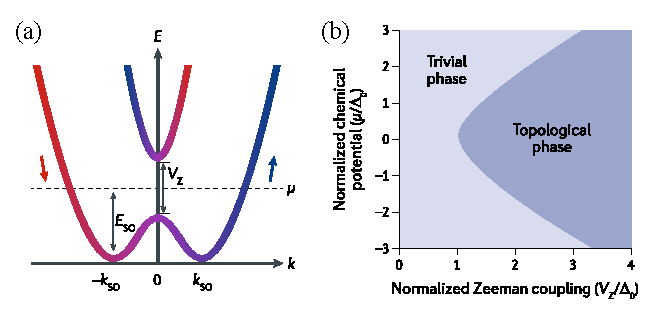
\includegraphics{04-Includes/Figures/intro1a.pdf}
    \caption
    [Spektrum energetyczne oraz topologiczny wykres fazowy dla nanodrutu półprzewodnikowego sprzężonego z nadprzewodnikiem~\cite{lutchyn.bakkers.2018}.]
    {Spektrum energetyczne oraz topologiczny diagram fazowy dla 1D układu.
    (a) Struktura pasmowa w funkcji pędu $k$ w obecności sprzężenia spin--orbita (\acrshort{SO}) oraz zewnętrznego pola magnetycznego $\zeeman$.
    Elektrony w~układzie posiadają paraboliczną relację dyspersyjną, która przy braku \acrshort{SO} oraz zewnętrznego pola magnetycznego jest zdegenerowana ze względu na spin elektronów.
    Sprzężenie \acrshort{SO} znosi degenerację poprzez ,,przesunięcie'' relacji dyspersyjnych o pęd $k_{SO}$ wprowadzając nową skalę energetyczną $E_{SO}$.
    Przyłożenie zewnętrznego pola magnetycznego powoduje otwarcie szczeliny energetycznej dla $k=0$.
    Jeśli poziom Fermiego $\muuniform$ (przerywana linia) znajduje się wewnątrz tej szczeliny, możliwe jest parowanie cząstek w ramach jednego pasma (tj. parowanie typu $p$). 
    (b) Przejście układu do fazy topologicznej (gdzie można oczekiwać realizacji \MZM\ na brzegu układu) określony jest ściśle przez wartości przez $\muuniform$ oraz $\zeeman$.
    Dla ustalonego $\muuniform$, pole magnetyczne musi przekroczyć pewną krytyczną wartość $V_Z^c = \sqrt{ \muuniform^2 + \DeltaSCuniform_0^2 }$ (granica reprezentowana przez ,,parabole'' na prawym panelu), gdzie $\DeltaSCuniform_0$ oznacza szczelinę nadprzewodzącą, np. wyindukowaną poprzez efekt bliskości z nadprzewodnikiem.
    Źródło:~\cite{lutchyn.bakkers.2018}.}
    \label{fig:intro1}
\end{figure}



\ornament


\section{Realizacja eksperymentalna}
\label{sec:signatures}


Współczesny rozwój technik eksperymentalnych umożliwił rozpoczęcie prac nad praktyczną realizacją systemów fizycznych, w których możliwa byłaby obserwacja \MZM.
W powyższych rozważaniach teoretycznych \MZM\ były realizowane w skończonym układzie 1D, w którym współistnieje sprzężenie \acrshort{SO} oraz nadprzewodnictwo, natomiast poziom Fermiego znajduje się blisko dna pasma --- rysunek~\ref{fig:intro1}(a).
Dzięki postępowi w realizacji niskowymiarowych struktur w skali atomowej, w ostatnich latach udało się zrealizować wiele eksperymentów w których uważa się, że realizowane są \MZM.
Eksperymenty te realizowane są w~hybrydowych nanostrukturach typu nadprzewodnik--półprzewodnik~\cite{deng.yu.2012,mourik.zuo.2012,das.ronen.2012,finck.vanharlingen.2013,nichele.drachmann.2017,gul.zhang.2018,deng.vaitiekenas.2016,gazibegovic.car.2017,deng.vaitiekenas.2018,zhang.liu.2018,wang.kong.2018},
w~jednowymiarowych monoatomowych łańcuchach atomów ferromagnetycznych na powierzchni nadprzewodników~\cite{nadj-perge.drozdov.2014,pawlak.kisiel.2016,feldman.randeria.2016,ruby.heinrich.2017,jeon.xie.2017,kim.palaciomorales.2018},
w wirach w nadprzewodnikach~\cite{sun.jia.2017,machida.sun.2019,jiang.dai.2019,chiu.machida.2019},
czy też w dwuwymiarowych nanostrukturach topologicznych ~\cite{menard.guissart.2017,palaciomorales.mascot.2018}.
Poniżej pokrótce przybliżono część z wymienionych układów.


\begin{SCfigure}
    \centering
    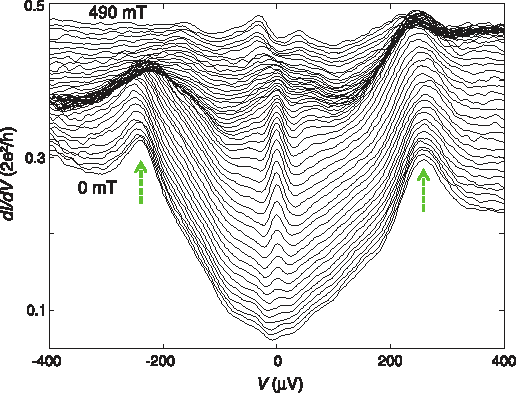
\includegraphics{04-Includes/Figures/Observe/observe1.pdf}
    \caption
    [Przewodność różniczkowa $\text dI/\text dV$  w funkcji napięcia $V$~\cite{mourik.zuo.2012}.]
{
    Przewodność różniczkowa $\text dI/\text dV$  w funkcji napięcia $V$ w układzie nanodrutu wykonanego z antymonku indu (InSb) połączonego z normalną (Au) i nadprzewodzącą (NbTiN) elektrodą. Wyniki w temperaturze $70$~mK. Zielone strzałki wskazują piki koherentne związane z trywialną szczeliną nadprzewodzącą, wyindukowaną w układzie poprzez efekt bliskości nadprzewodnika.
    Źródło:~\cite{mourik.zuo.2012}.
}
    \label{fig:observe1}
\end{SCfigure}


%\subsection*{Realizacja MZM w~układach hybrydowych}
\subsection*{Układy hybrydowe}


Warunki do bezpośredniej realizacji modelu Kitaeva, opisane powyżej, mogą zostać spełnione w układach hybrydowych --- rysunek~\ref{fig:observe4} (zaczerpnięty z pracy~\cite{zhang.liu.2018}).
Dla przykładu w nanodrutach wykonanych z antymonku indu (InSb) czy antymonku arsenu (InAs)
%, gdzie energia związana z efektem sprzężenia \acrshort{SO} wynosi $E_{SO}=0.05\div 1$~meV
~\cite{mourik.zuo.2012,vanweperen.tarasinski.2015,shabani.kjaergaard.2016,lutchyn.bakkers.2018} sprzężonych z nadprzewodnikiem. 
%W nanodrutach, wykonanych z wymienionych materiałów, po dodaniu podłoża nadprzewodzącego, indukowana jest szczelina nadprzewodząca $\DeltaSCuniform_0$ wynikająca z efektu bliskości nadprzewodnika.
Sprzężenie \acrshort{SO} oraz niska koncentracja nośników jest cechą wewnętrzną tych materiałów, tj. półprzewodników.
Z kolei efekt bliskości z nadprzewodnikiem, powoduje, że indukowana jest szczelina nadprzewodząca $\DeltaSCuniform_0$.
Przykładowo, w materiale InSb pokrytym NbTiN indukowana jest szczelina $\DeltaSCuniform_0=0.65$~meV~\cite{gul.zhang.2018}, a pokrytym Al $\DeltaSCuniform_0=0.2$~meV~\cite{zhang.liu.2018}.
%W przypadku InAs pokrytym Al wyindukowana szczelina wynosi $\DeltaSCuniform_0=0.2$~meV~\cite{deng.vaitiekenas.2018}.
Oddziaływanie \acrshort{SO}, wraz z wyindukowaną szczeliną nadprzewodzącą $\DeltaSCuniform_0$, stwarzają warunki obserwacji \MZM\ w wymienionych materiałach.


Obecność \MZM\ powinna być możliwa do obserwacji w pomiarach transportowych, tj. przewodności różniczkowej $\conductance (V) = dI/dV$.
W tym przypadku, \MZM\ mogą być wykryte w eksperymentach transportowych jako piki w $\conductance$ przy zerowym napięciu ($V=0$)~\cite{mourik.zuo.2012}.
W pracy~\cite{mourik.zuo.2012} dokonywano pomiarów $\conductance$ dla nanodrutów wykonanych z antymonku indu (InSb) połączonych z normalną i nadprzewodzącą elektrodą.
W zerowej temperaturze, w odróżnieniu od stanów trywialnych, obecność \MZM\ powinna objawiać się pikiem przy braku napięcia ($V=0$) w przewodności różniczkowej $\conductance = 2 \conductance_0$~\cite{flensberg.2010,prada.san-jose.2012,stanescu.tewari.2012,liu.potter.2012,rainis.trifunovic.2013,lutchyn.bakkers.2018}, gdzie $\conductance_0=e^2/h$ jest kwantem przewodnictwa, $e$ to ładunek elementarny, a $h$ to stała Plancka.
Jest to związane ze zjawiskiem nazywanym \textit{odbiciem Andreeva}~\cite{law.lee.2009,he.ng.2014}.
W przypadku wspomnianego eksperymentu, elektrony, które tunelują z elektrody do układu hybrydowego, sprzęgają się z \MZM, czyli stanami o zerowej energii.
Zarówno spin jak i prąd tunelowy, może stanowić proste narzędzie do wstępnej detekcji \MZM.
Potencjał bariery można kontrolować przy pomocy przyłożonego napięcia $V$.
Teoretycznie, zmieniając pole magnetyczne można zmienić stan układu z \textit{fazy trywialnej} (gdzie nie występują \MZM) na \textit{fazę topologiczną}, w której występują \MZM.
Dla wartości pola magnetycznego około $100$~mT, zaobserwowano stany wewnątrz szczeliny o zerowej energii (przy braku napięcia $V=0$) ---  rysunek~\ref{fig:observe1} (zaczerpnięty z pracy~\cite{mourik.zuo.2012}).
Jest to jedna z pierwszych prac w której dokonane obserwacje mogą przypuszczalnie potwierdzać hipotezę realizacji quasicząstek \MZM\ w takich układach.


W pracy~\cite{zhang.liu.2018} autorzy jako jedni z pierwszych pokazują kwantyzację przewodności różniczkowej $G$ w omawianych układach.
W tych badaniach wykorzystano nanodruty półprzewodnikowe wykonane z SbIn, pokrytego warstwą nadprzewodzącego Al.
Zrealizowany układ pomiarowy wraz ze schematyczną ilustracją, pokazano na rysunku~\ref{fig:observe4}(a).
Rysunek~\ref{fig:observe4}(b)--(d) pokazuje porównanie wyników eksperymentalnych oraz teoretycznych.
W~zakresie wartości pola magnetycznego od około $0.8$ do $0.9$ T widać, że wartość $\conductance (V=0)$ jest równa w przybliżeniu $2 \conductance_0$, co potwierdzało by realizację \MZM.


\begin{figure}
    \centering
    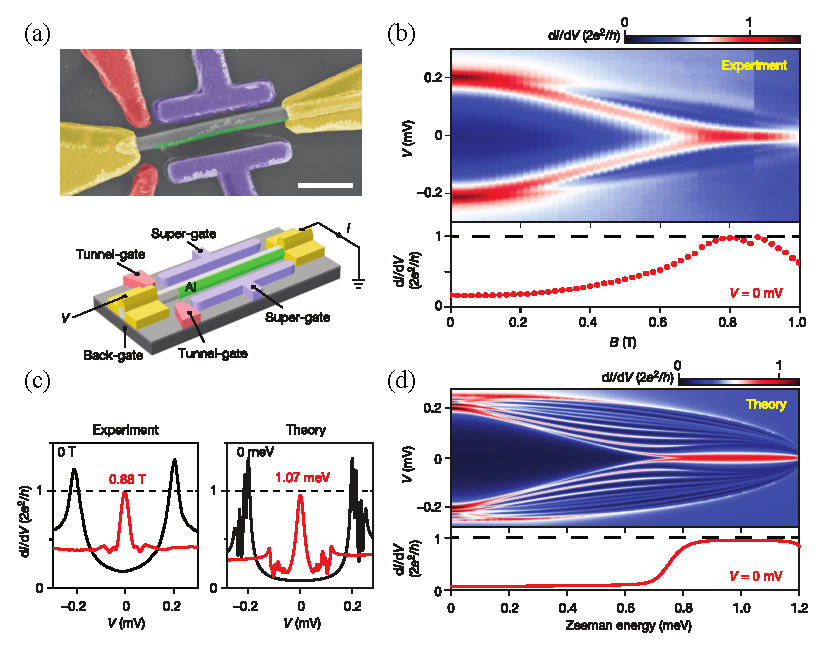
\includegraphics[width=0.9\textwidth]{04-Includes/Figures/Observe/observe4.pdf}
    \caption
    [Układ pomiarowy oraz przewodność różniczkowa -- porównanie wyników doświadczalnych z numerycznymi~\cite{zhang.liu.2018}.]
{%
    (a) Obraz ze skaningowego mikroskopu elektronowego układu pomiarowego wraz z przedstawionym schematem.
    Nanodrut wykonany z InSb (kolor szary) częściowo pokryty cienką warstwą nadprzewodzącego aluminium (kolor zielony).
    Bramki tunelowe zaznaczono kolorem różowym, kolorem fioletowym zaznaczono ,,super'' bramki za pomocą których można kontrolować potencjał chemiczny w układzie.
    Złącza elektryczne wykonane z Cr/Au zaznaczono kolorem żółtym.
    (b) Wyniki pomiarów przewodności różniczkowej $dI/dV$ w funkcji napięcia $V$ oraz pola magnetycznego $B$ (energii Zeemana).
    (c-d) Porównanie eksperymentalnej oraz teoretycznej przewodności różniczkowej $dI/dV$.
    Wyniki przedstawione na (b) i (d) jakościowo są zgodne.
    Nie są jednak zgodne dokładnie co wynika z dokładności eksperymentu oraz z nieznanych dokładnych wartości parametrów potrzebnych do % wykorzystanych w 
    lepszej symulacji modelu.
    Źródło:~\cite{zhang.liu.2018}.
}
    \label{fig:observe4}
\end{figure}

\begin{SCfigure}
    \centering
    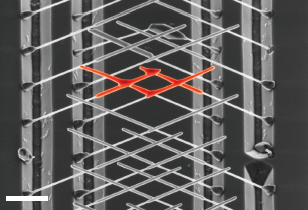
\includegraphics[width=0.5\textwidth]{04-Includes/Figures/Observe/observe5.png}
    \caption
    [Zdjęcie ze skaningowego mikroskopu elektronowego struktury 4 nanodrutów~\cite{gazibegovic.car.2017}.]
    {
    Zdjęcie ze skaningowego mikroskopu elektronowego struktury 4 nanodrutów InSb z naniesioną warstwą nadprzewodzącą Al (zaznaczono czerwonym kolorem). 
    Skala (lewy dolny róg) odpowiada $1$ {\textmu}m, skanowanie dokonano pod kątem $30^\circ$.
    Źródło:~\cite{gazibegovic.car.2017}.
    }
    \label{fig:observe5}
\end{SCfigure}



Należy tutaj podkreślić, że wartość piku $\conductance (V=0)$, nie jest jednoznaczną informacją odnośnie obecności \MZM\ w układzie.
Podczas analizy takich wyników należy zachować szczególną ostrożność, ponieważ źródłem takiego piku może być np. efekt Kondo~\cite{zazunov.plugge.2018},
stany brzegowe Andreeva~\cite{mourik.zuo.2012,moore.stanescu.2018,hell.flensberg.2018,liu.sau.2018,lai.sau.2019,yavilberg.ginossar.2019,danon.hellenes.2020},
nieporządek~\cite{liu.potter.2012,tuovinen.perfetto.2019}
lub wygładzony potencjał na brzegu nanodrutu~\cite{kells.meidan.2012}.

Do eksperymentów związanych z wyplataniem cząstek \MZM\ jeszcze daleka droga, jednak poczyniono w tym kierunku znaczące postępy.
W pracy~\cite{gazibegovic.car.2017} autorzy przedstawili technikę epitaksji umożliwiającą konstrukcję sieci nanodrutów.
Konstrukcja sieci kilku nanodrutów, jest kluczowa dla procesu wymiany \MZM.
Na rysunku~\ref{fig:observe5} (zaczerpniętym z pracy~\cite{gazibegovic.car.2017}) przedstawiono zdjęcie ze
skaningowego mikroskopu elektronowego.
Rysunek przedstawia otrzymaną przez autorów pracy strukturę czterech nanodrutów InSb pokrytych nadprzewodzącą warstwą Al (zaznaczone kolorem czerwonym).
Ostateczna eksperymentalna weryfikacja \MZM\ odbędzie się wraz z wykazaniem \acrshort{NAS}.
Takie struktury mogą służyć do sterowania położenia \MZM\ za pomocą potencjału chemicznego $\muuniform$ lub pola magnetycznego $B$~\cite{alicea.oreg.2011}.
Modyfikując $\muuniform$ lub $B$ można kontrolować wielkość obszaru topologicznego w obrębie nanodrutu, co w konsekwencji może prowadzić do wymiany \MZM.
Okazuje się, że taka wymiana cząstek nie musi być zrealizowana za pomocą bezpośredniej manipulacji pozycji quasicząstek.
Wyplatanie może przebiegać z~wykorzystaniem efektywnego przesunięcia \MZM, z~wykorzystaniem tzw. schematu \textit{measurement-only}~\cite{bonderson.freedman.2008,bonderson.freedman.2009}, który bazuje na serii pomiarów --- kwantowej teleportacji informacji.
Takie pomiary mogą zostać zrealizowane z wykorzystaniem kontroli strumienia pola magnetycznego pomiędzy dwoma złączami Josephsona~\cite{hyart.vanheck.2013,vijay.fu.2016,aasen.hell.2016,plugge.rasmussen.2017}, na których spoczywa układ zawierający \MZM.
Zasadniczą przewagą takiego rozwiązania jest fakt, że w celu wykonania wyplatania \MZM\ nie trzeba korzystać z modyfikacji lokalnych potencjałów $\muuniform$ czy lokalnego pola $B$. 
Zmiany takich lokalnych parametrów mogą być wrażliwe na problemy związane z~nieporządkiem czy niedokładnością aparatury, co zostaje całkowicie wyeliminowane w podejściu z wykorzystaniem schematu kontroli strumienia.

%\subsection*{Realizacja MZM w~łańcuchach magnetycznych}
\subsection*{Ferromagnetyczne łańcuchy monoatomowe}

\begin{SCfigure}
    \centering
    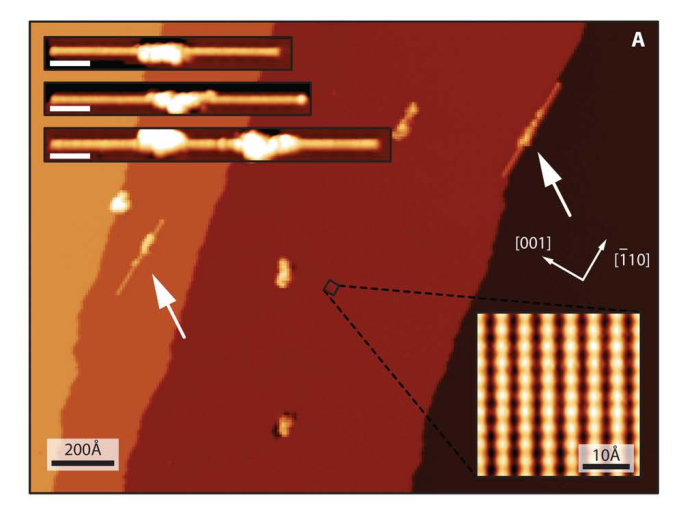
\includegraphics[width=0.5\textwidth]{04-Includes/Figures/Observe/observe2.pdf}
    \caption
    [Topografia nadprzewodzącego ołowiu Pb, z naniesionymi 3 nanodrutami żelaza Fe~\cite{nadj-perge.drozdov.2014}.]
    {Topografia powierzchni ołowiu Pb, z naniesionymi 3 nanodrutami żelaza Fe. 
    Wyspy oraz łańcuchy wyhodowane na powierzchni zaznaczone są białym kolorem.
    Atomowo czyste tarasy Pb to obszary zaznaczone tym samym kolorem (żółty, pomarańczowy, jasnobrązowy, ciemnobrązowy).
    Wstawka w prawym dolnym rogu prezentuje anizotropową strukturę powierzchni Pb$(110)$.
    Wstawki w lewym górnym rogu prezentują zdjęcia kilku łańcuchów Fe oraz wysp z których ,,wyrosły'' (skala $50$ \AA).
    Źródło:~\cite{nadj-perge.drozdov.2014}.
    }
    \label{fig:observe2}
%\end{figure}
%\begin{figure}
\end{SCfigure}
\begin{SCfigure}

%\vspace{1cm}

    \centering
    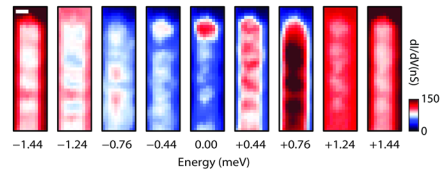
\includegraphics[width=0.5\textwidth]{04-Includes/Figures/Observe/observe3a.png}
    \caption
    [Przestrzenna i energetyczna przewodność różniczkowa $G=\text dI/\text dV$~\cite{nadj-perge.drozdov.2014}.]
    {Przestrzenna i energetyczna przewodność różniczkowa $\conductance=\text dI/\text dV$. Temperatura w jakiej dokonywano pomiaru: $1.4$~K.
    Skala: biała linia odpowiada długości $10$~\AA.
    Źródło:~\cite{nadj-perge.drozdov.2014}.
    }
    \label{fig:observe3}
\end{SCfigure}

Innym przykładem, gdzie oczekuje się realizacji \MZM, są monoatomowe łańcuchy na powierzchni nadprzewodnika.
Dla przykładu w pracy~\cite{nadj-perge.drozdov.2014} autorom udało się wytworzyć ferromagnetyczne łańcuchy atomowe żelaza (Fe) na powierzchni nadprzewodzącego ołowiu (Pb).
Topografię układu pomiarowego można zobaczyć na rysunku~\ref{fig:observe2} (zaczerpnięty z pracy~\cite{nadj-perge.drozdov.2014}).
Na wyraźnie widocznych tarasach Pb, widać nanodruty Fe (oznaczone poprzez białe strzałki oraz wstawki w lewym górnym rogu rysunku~\ref{fig:observe2}).
Stosując technikę wysokorozdzielczej spektroskopii obrazowej
zmierzono lokalną przewodność różniczkową $\conductance$ w funkcji energii --- rysunek~\ref{fig:observe3} (zaczerpnięty z pracy~\cite{nadj-perge.drozdov.2014}).
Dla zerowej energii, widać wzbudzenie znajdujące się na końcu nanodrutu.
To wzbudzenie może być interpretowane jako \MZM.
Dla pozostałych energii można zaobserwować stany zdelokalizowane w obrębie całego łańcucha.
Te mapy mogą również posłużyć do badania zanikającego rozkładu przestrzennego \MZM\ od brzegów nanodrutu.
Zmierzona długość lokalizacji \MZM\ była rzędu $10$ w porównaniu do odległości od brzegu nanodrutu do środka wyspy, z~której został stworzony.
Z uwagi na efekty termiczne ($1.4$ K), pik w zerowej energii w przewodności różniczkowej dla tego eksperymentu był poszerzony, co w konsekwencji doprowadziło do otrzymania $\conductance= 1.3\cdot 10^{-4} \conductance_0$,  zdecydowanie odbiegającej od idealnej wartości $2\conductance_0$.
Efekty termiczne lub nieporządek mogą prowadzić do ,,niekwantowania'' piku $\conductance$~\cite{stanescu.2016}, co sprawia, że pomiar $\conductance$ w celu identyfikacji \MZM\ może być trudny w interpretacji.


\subsection*{Podsumowanie}
Należy tutaj podkreślić, że żadna z~wymienionych powyżej prac doświadczalnych nie udowodniła istnienia \MZM\ w  sposób jednoznaczny.
Dowodem takim mógłby być pomiar potwierdzający, że obserwowane stany podlegają statystyce nieabelowej.
Wymagane są zatem eksperymenty wyplatania (ang. \textit{braiding}) lub niedawno zaproponowane \textit{eksperymenty słabego pomiaru}~\cite{manousakis.wille.2020}.
Te ostatnie eksperymenty polegają na pomiarach 
strzałowego szumu korelacji krzyżowej (ang. \textit{cross-correlation shot noise}).
W pracy~\cite{manousakis.wille.2020} pokazano, że sygnatura \MZM\ może zostać wyekstrahowana z takiego szumu w układzie połączonych nanodrutów.
Cytowane prace, kolejne realizowane oraz planowane badania, zbliżają nas jednak do weryfikacji obecności \MZM.
%Postęp w~ostatnich latach jest relatywnie duży, ale wciąż jest to początek \textit{dalekiej wędrówki} w~kierunku konstrukcji topologicznego komputera kwantowego.
%Poniżej streszczono wyniki jednych z~ważniejszych prac doświadczalnych ostatnich 10-ciu lat w dziedzinie związanej z \MZM\ ~\cite{mourik.zuo.2012,nadj-perge.drozdov.2014,gazibegovic.car.2017,zhang.liu.2018}.
Prezentowane wyniki należy zatem traktować, jako pierwszą fazę podstawowych badań eksperymentalnych.
Jest to dopiero pierwszy kamień milowy, w bardzo długiej wędrówce w kierunku konstrukcji pierwszego działającego topologicznego komputera kwantowego.
Obserwacja \acrshort{NAS} jest również kluczowa do ostatecznej weryfikacji obecności \MZM\ w układach kwantowych.


\ornament


\section{Badania teoretyczne}
\label{sec:theoreticalPerspectives}

Badania teoretyczne, prowadzone równolegle do prac eksperymentalnych, relatywnie dobrze odtwarzają wyniki pomiarów na poziomie jakościowym (czasem nawet ilościowym) --- np. prezentowany wcześniej rysunek~\ref{fig:observe4}.
Modele opisujące realizowane układy głównie bazują na układach 1D.
%W pierwszym kwantowaniu układ takie może być w prosty sposób opisany hamiltonianem~\cite{liu.sau.2017}:
%\begin{equation}
%\hatH_{\text{1D}} = \left( -\frac{\HBAR}{2\mass^{\ast}} \partial_{x}^{2} - \iu %\alpha_{R} \partial_{x} \paulii_{y} - \muuniform \right) \pauliiParticle_{z} + %\zeeman \paulii_{x} + \DeltaSCuniform_{0} \pauliiParticle_{z} ,
%\end{equation}
%gdzie $\mass^{\ast}$ jest masą efektywną elektronów, $\alpha_{R}$ opisuje sprzężenie \acrshort{SO}, $\zeeman$ opisuje rozszczepienie Zeemana, natomiast $\DeltaSCuniform_{0}$ jest wyindukowaną szczeliną nadprzewodzącą. 
%Macierze $\paulii$ oraz $\pauliiParticle$ oznaczają tutaj macierze Pauliego, działające odpowiednio w przestrzeni spinów oraz przestrzeni cząstka--dziura.
%Powyższy zapis jest równoznaczny do zapisu w języku ,,drugiego kwantowania'', który stosowany jest w dalszej części prezentowanej rozprawy.\footnote{Szczegółowy opis mikroskopowy hamiltonianu w~formalizmie drugiej kwantyzacji można znaleźć w sekcji~\ref{sec:kitaev} oraz~\ref{sec:fullHamiltonianConstruction}.}
W drugim kwantowaniu taki układ może być opisany przez następujący minimalny model
\begin{align}
    \hatH_{\text{1D}} =& \underbrace{\sum_{ ij\sigma}\left( - \t0 - \muuniform\deltaij\right)\aisd\ajs}_{\hatH_{\text{free}}}
    -
     \underbrace{ h \sum_{i\sigma\sigma'} \aisd ( \paulii^{z} )_{\sigma\sigma'}\,  \aisp}_{\hatH_{\text{mag}}}
     +\nonumber\\
     & \underbrace{\alpha^R \sum_{i\sigma\sigma'} \left( \aisd (\iu\paulii^{y} )_{\sigma\sigma'}\, a_{i+1,\sigma'} + \hc \right) }_{\hatH_{SO}} +
     \underbrace{\sum_{i}\left( \DeltaSCuniform \aidu\aidd + \hc\right)}_{\hatH_{\text{prox}}},
\end{align}
gdzie $\aisd$ oraz $\ais$ to odpowiednio operator kreacji i anihilacji fermionu o spinie $\sigma=\{\uparrow,\downarrow\}$ w~węźle $i$,
$\paulii^{x,y,z}$ to macierze Pauliego,
$\tuniform$ to całka przeskoku ($\t0 = 1$ w przypadku przeskoku pomiędzy najbliższymi sąsiadami oraz $0$ w innych przypadkach),
$\muuniform$ to potencjał chemiczny,
$h$ to pole magnetyczne równoległe do drutu,
$\alpha^{R}$ opisuje sprzężenie \acrshort{SO} typu Rashba,
a $\DeltaSCuniform$ to szczelina nadprzewodząca (wyindukowana w drucie przez efekt bliskości z nadprzewodnikiem).
Hamiltonian $\hatH_{\text{free}}$ opisuje elektrony swobodne w układzie 1D, $\hatH_{\text{mag}}$ wpływ zewnętrznego pola magnetyczne na elektrony (efekt Zeemana), $\hatH_{SO}$ opisuje \acrshort{SO} typu Rashba, natomiast $\hatH_{\text{prox}}$ opisuje nadprzewodnictwo.
Relatywna łatwość formułowania problemu badawczego w takim formalizmie stwarza sprzyjające warunki do rozwoju badań teoretycznych, mających na celu opis układów zrealizowanych eksperymentalnie~\cite{lutchyn.sau.2010,oreg.refael.2010,klinovaja.stano.2012,karzig.refael.2013,rainis.trifunovic.2013,li.chen.2014,vernek.penteado.2014,wakatsuki.ezawa.2014,heimes.mendler.2015,ruiz-tijerina.vernek.2015,maska.gorczyca.2017,maska.domanski.2017,ptok.kobialka.2017,liu.sau.2017,prada.aguado.2017,chevallier.szumniak.2018,padavic.hegde.2018,alecce.dellanna.2017,gau.plugge.2018,hua.chen.2019,kobialka.sedlmayr.2019,kobialka.ptok.2019,kobialka.domanski.2019,wille.egger.2019,schulenborg.flensberg.2020} oraz zagadnień związanych z ogólnie rozumianą informatyką kwantową bazującą na \MZM\ ~\cite{alicea.oreg.2011,vanheck.akhmerov.2012,fulga.vanheck.2013,vanheck.hyart.2015,karzig.oreg.2016,sekania.plugge.2017},


O ile w przypadku układów hybrydowych sprzężenie \acrshort{SO} jest cechą wewnętrzną układu, o tyle w przypadku łańcuchów magnetycznych pokazano, że porządek magnetyczny może prowadzić do efektów podobnych, wytwarzając efektywne oddziaływanie \acrshort{SO}.
Pokazano to w licznych badaniach uwzględniających mechanizm RKKY~\cite{braunecker.simon.2013,pientka.glazman.2013,klinovaja.stano.2013,kim.cheng.2014,braunecker.simon.2015,choy.edge.2011,nadj-perge.drozdov.2013}
W takim układzie, helikalny porządek magnetyczny wynika z minimalizacji energii układu oraz w istotny sposób wpływa na zakres istnienia fazy topologicznej~\cite{gorczyca-goraj.domanski.2019}. 
Okazuje się, że w takich układach, jedną z sygnatur \MZM\ może być ich polaryzacja spinowa~\cite{maska.gorczyca.2017,maska.domanski.2017}.
Prezentowane wyniki obliczeń modelują wyniki jakie można otrzymać za pomocą spektroskopii SESAR (ang. \textit{selective equal--spin Andreev spectroscopy}).
Otrzymane teoretyczne wyniki są jakościowo zgodne z wynikami eksperymentalnymi przedstawionymi w pracy \cite{jeon.xie.2017}.


\subsection*{Wpływ oddziaływań wielociałowych}

W kontekście praktycznej implementacji \MZM\ w obliczeniach kwantowych, oddziaływania wielociałowe mogą odgrywać bardzo istotną rolę.
Dla przykładu, średnie oddziaływania mogą prowadzić do stabilizacji \MZM\ w układach kwantowych~\cite{stoudenmire.alicea.2011,hassler.schuricht.2012,katsura.schuricht.2015,gergs.niklas.2016,dominguez.cayao.2017}.
Badania oddziaływania kulombowskiego (odpychania na węźle) w przypadku fermionów o spinie połówkowym prowadzone były w przybliżeniu Hartree--Focka~\cite{stoudenmire.alicea.2011,manolescu.marinescu.2014}.
Oddziaływanie takie prowadzi do obniżenia krytycznego pola magnetycznego, wymaganego do wytworzenia \MZM\ w układzie, oraz może prowadzić do stabilizacji \MZM~\cite{peng.pientka.2015,dominguez.cayao.2017}.
Natomiast w przypadku układów bezspinowych fermionów, oddziaływania pomiędzy najbliższymi sąsiadami były zbadane z wykorzystaniem techniki 
\glslink{DMRG}{grupy renormalizacji macierzy gęstości (ang. density matrix renormalization group, DMRG)}~\cite{thomale.rachel.2013,gergs.niklas.2016,miao.jin.2018}
oraz \glslink{ED}{dokładnej diagonalizacji (ang. exact diagonalization, ED)}~\cite{ng.2015}. 
W~takim przypadku, średnie oddziaływania mogą stabilizować porządek topologiczny.


Model Kitaeva z oddziaływaniami wielociałowymi pomiędzy najbliższymi sąsiadami  w~punkcie symetrycznym\footnote{Punkt symetryczny oznacza tutaj parametry $\DeltaSCuniform=\tuniform$ i~$\muuniform=0$. Szczegóły modelu Kitaeva zostały opisane w~sekcji~\ref{sec:kitaev}.} udało się rozwiązać dokładnie~\cite{miao.jin.2017}, wykorzystując do tego transformację Jordana--Wignera~\cite{jordan.wigner.1928} i operacje obrotów spinów.
Punkt symetryczny jest szczególnym przypadkiem tego modelu, który w przypadku braku oddziaływań w prosty sposób można rozwiązać analitycznie, co zostało przedstawione w sekcji~\ref{sec:kitaev}.
W takim wypadku, \MZM\ są całkowicie zlokalizowane na pojedynczym węźle sieci, mają niekończony czas życia, nawet w~przypadku skończonego rozmiaru układu.

\begin{figure}
    \centering
    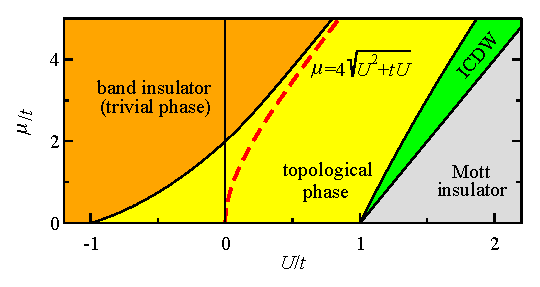
\includegraphics{04-Includes/Figures/Theory/theory1.pdf}
    \caption[Diagram fazowy modelu Kitaeva z oddziaływaniami wielociałowymi pomiędzy najbliższymi sąsiadami. Źródło:~\cite{katsura.schuricht.2015}]
   {Diagram fazowy modelu Kitaeva z oddziaływaniami wielociałowymi pomiędzy najbliższymi sąsiadami dla szczególnych parametrów modelu $\DeltaSCuniform=\tuniform$, w funkcji potencjału chemicznego $\muuniform$ oraz oddziaływania $U$. Kolor pomarańczowy: faza trywialna, kolor żółty: faza topologiczna, kolor zielony: faza niewspółmiernych fal gęstości ładunku (ang. \textit{incommensurate charge density wave, ICDW}), kolor szary: izolator Motta.
   Czerwoną przerywaną linią zaznaczono zakres parametrów, dla których możliwe jest dokładne rozwiązanie.
   Źródło:~\cite{katsura.schuricht.2015}.}
    \label{fig:theory1}
\end{figure}

Model Kitaeva z oddziaływaniami pomiędzy najbliższymi sąsiadami można również rozwiązać w przypadku wybrania specyficznych lokalnych potencjałów chemicznych w funkcji pozostałych parametrów modelu, co zostało pokazane w pracy~\cite{katsura.schuricht.2015}.
Zakres parametrów dla których możliwe jest takie analityczne rozwiązanie zaznaczono czerwoną linią na rysunku~\ref{fig:theory1} (zaczerpnięty z pracy~\cite{katsura.schuricht.2015}).
Na rysunku~\ref{fig:theory1} przedstawiono schematyczny wykres fazowy dla modelu Kitaeva z oddziaływaniami pomiędzy najbliższymi sąsiadami dla symetrycznego punktu w funkcji potencjału chemicznego $\muuniform$ oraz oddziaływania\footnote{Relacja pomiędzy potencjałem $U$, a przyjętą w~tej pracy notacją $\Vuniform$ jest następująca $U=4\Vuniform$.} $U$.
Rozważania dotyczą, jednorodnego łańcucha Kitaeva, o otwartych warunkach brzegowych.
Faza topologiczna, w~której w układzie mogą znajdować się \MZM, zaznaczona kolorem żółtym, ulega powiększeniu ze względu na potencjał chemiczny $\muuniform$ wraz ze wzrostem oddziaływania $U$.

\begin{SCfigure}
    \centering
    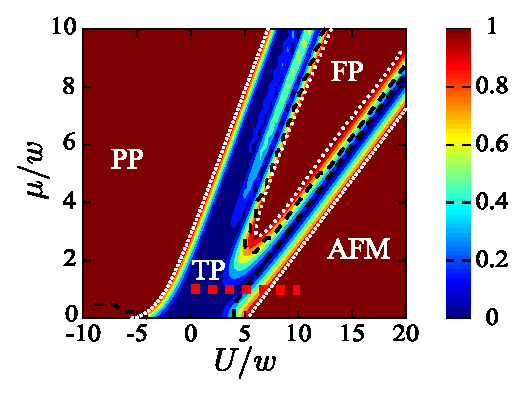
\includegraphics{04-Includes/Figures/Theory/theory2.pdf}
    \caption[Degeneracja stanu podstawowego. Źródło:~\cite{ng.2015}]
   {Degeneracja stanu podstawowego w modelu Kitaeva z oddziaływaniami wielociałowymi pomiędzy najbliższymi sąsiadami w funkcji potencjału chemicznego $\muuniform$ oraz oddziaływania $U$. 
   Na rysunku oznaczono fazy: 
   fazę topologiczną (ang. \textit{topological phase, TP}),
   fazę ferromagnetyczną (ang. \textit{ferromagnetic phase, FP}),
   fazę antyferromagnetyczą (ang. \textit{antiferromagnetic phase, AFP}),
   fazę trywialną (ang. \textit{trivial phase, PP}).
      Źródło:~\cite{ng.2015}.}
    \label{fig:theory2}
\end{SCfigure}

Jednym z warunków koniecznych istnienia \MZM\ w układach, jest degeneracja stanu podstawowego $\deltaE$ pomiędzy dwoma sektorami parzystości, nie jest to natomiast warunek wystarczający dla obecności \MZM.
W pracy~\cite{ng.2015} zbadano proces dekoherencji w łańcuchu Kitaeva z oddziaływaniami pomiędzy najbliższymi sąsiadami.
Na rysunku~\ref{fig:theory2} (zaczerpniętym z pracy~\cite{ng.2015}) przedstawiono otrzymane wyniki $\deltaE$ z pracy~\cite{ng.2015}.
Niebieski kolor odpowiada wartościom $\deltaE=0$, czyli potencjalnemu obszarowi występowania \MZM.\footnote{W rozdziale~\ref{chap:identification} odtworzono te wyniki oraz odpowiednio skomentowano.}
%Podczas analizy takich wyników należy zachować szczególną czujność.
%W rozdziale~\ref{chap:identification} odtworzono te wyniki i odpowiednio skomentowano.
Obszar występowania \MZM\ w takim układzie jest zdecydowanie mniejszy, niż obszar oznaczony kolorem niebieskim.

\begin{SCfigure}
    \centering
    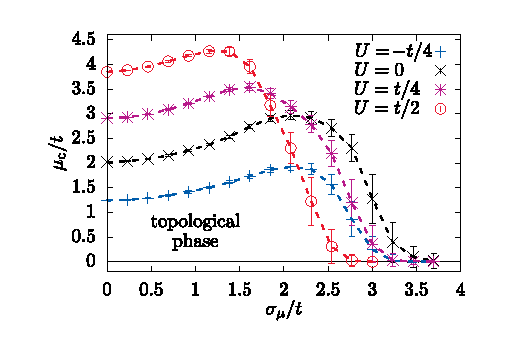
\includegraphics{04-Includes/Figures/Theory/theory3.pdf}
    \caption[Wpływ oddziaływań pomiędzy najbliższymi sąsiadami $U$ oraz nieporządku $\sigma_\mu$ na granice obszaru topologicznego w modelu Kitaeva.]
   {Wpływ oddziaływań pomiędzy najbliższymi sąsiadami $U$ oraz nieporządku $\sigma_\mu$ na granice obszaru topologicznego w modelu Kitaeva. 
   Punkt symetryczny $\DeltaSCuniform=\tuniform$.
   Źródło:~\cite{gergs.fritz.2016}.}
    \label{fig:theory3}
\end{SCfigure}

Korzystając z metody \acrshort{DMRG}, autorzy pracy~\cite{gergs.fritz.2016} badali wpływ oddziaływań pomiędzy najbliższymi sąsiadami i nieporządku na obecność fazy topologicznej w łańcuchu Kitaeva.
Na rysunku~\ref{fig:theory3} (zaczerpniętym z pracy~\cite{gergs.fritz.2016}) przedstawiono granicę fazy topologicznej i trywialnej w funkcji potencjału chemicznego $\muuniform_c$ oraz nieporządku $\sigma_\mu$ dla kilku realizacji oddziaływania $U$.
Otrzymano standardowy wynik poszerzenia obszaru topologicznego ze względu na potencjał chemiczny wraz ze wzrostem oddziaływania $U$.
Wpływ nieporządku jest natomiast przeciwny -- powierzchnia obszaru topologicznego ze wzrostem $U$ maleje.
%Natomiast wraz ze wzrostem oddziaływania $U$, granica obszaru topologicznego ze względu na nieporządek maleje.
W pracy~\cite{gergs.fritz.2016} można znaleźć interesujące kryteria dotyczące identyfikacji obszaru topologicznego. 


%Omówione prace oraz wykorzystane w nich metody, w większości nie umożliwiają generowania rozkładu przestrzennego \MZM, metody są ograniczone do badania oddziaływań krótko zasięgowych, a wykorzystywane kryteria obecności \MZM\ nie są jednoznaczne. {\bf nieeeee wszystko jest cacy to jest genialne nie pisz o problemach ... nie tutaj}

\ornament

\section*{Cel pracy}

Ze względu na praktyczne zastosowania \MZM, istotne jest dokładne poznanie czynników wpływających na te stany. 
\MZM\ istnieją w układach niskowymiarowych.
W takich układach oddziaływania wielociałowe mogą posiadać kluczowe znaczenie  i są one słabo zbadane.
Ze względu na swój charakter, często tego zagadnienia nie można rozwiązać za pomocą rachunku zaburzeń i wymagane jest zastosowania zaawansowanych technik numerycznych.
W związku z powyższym, głównym celem prezentowanej rozprawy było:
\begin{itemize}
\item {\bf opracowanie metody numerycznej do badania wpływu oddziaływań wielociałowych na \MZM},
\item {\bf zastosowanie zaproponowanej metody do zbadania wpływu oddziaływań wielociałowych na operację wyplatania \MZM}.
\end{itemize}
W niniejszej pracy badam wpływ oddziaływań wielociałowych na \MZM\ w układach 1D opisanych modelem Kitaeva. 
Szczegółowy opis tego modelu został przedstawiony w~rozdziale~\ref{chap:majorana}, natomiast wykorzystywana metodologia badania zastosowań \MZM\ w obliczeniach kwantowych w~rozdziale~\ref{chap:topologicalQuantumComputing}.
Podstawowe aspekty związane z konstrukcją hamiltonianów w bazie Wanniera dla pełnej przestrzeni Hilberta przedstawiłem w rozdziale~\ref{chap:diagonalization}.
W~rozdziale~\ref{chap:LIOMs} zaprezentowałem zaproponowaną przez nas metodę, która umożliwia badanie \MZM\ w modelach zawierających dowolne oddziaływania wielociałowe.
%Metoda nie jest też ograniczona co do specyficznych parametrów układu.
Metoda jest ogólna i umożliwia generowanie struktury przestrzennej \MZM, bez względu na parametry układu czy obecność dowolnych oddziaływań wielociałowych.
Rozdział~\ref{chap:dynamics} dotyczy dynamiki kwantowej.
Przedstawiłem tutaj schematy numeryczne do rozwiązywania równania Schr\"odingera, również pod kierunkiem badań związanych z wyplataniem \MZM.
Obliczenia zostały wykonane z~wykorzystaniem metody dokładnej diagonalizacji.
W pierwszej kolejności (rozdział~\ref{chap:identification}), przetestowaliśmy algorytm poprzez identyfikację \MZM\ w rozszerzonym modelu Kitaeva o oddziaływania wielociałowe.
Następnie, zaproponowany algorytm wykorzystaliśmy do badania wpływu dalekozasięgowych oddziaływań na czasy życia oraz strukturę przestrzenną \MZM\ (rozdział~\ref{chap:longrange}).
Na koniec, zbadaliśmy operację wyplatania \MZM\ oraz wpływ oddziaływań na ten proces (rozdział~\ref{chap:phaseGate}).
Ponadto, zaproponowaliśmy również nową bramkę fazową dla qubitu bazującego na \MZM.
Zaproponowana bramka fazowa, w odróżnieniu od standardowej bramki fazowej bazującej na fazie dynamicznej, bazuje na fazie geometrycznej.
Jest to szczególnie ważne, ponieważ faza geometryczna nie zależy bezpośrednio od czasu. 
W takiej bramce fazowej faza, jaką nabierze qubit, zależeć będzie tylko i wyłącznie od zmian parametrów hamiltonianu.
Bramka fazowa bazująca na fazie geometrycznej powinna posiadać mniejszy błąd względem realizacji bramki fazowej na bazie fazy dynamicznej.

\ornament
